\begin{figure}[h]
	\centering
	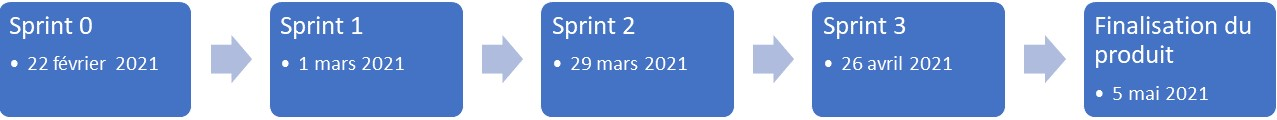
\includegraphics[width=\textwidth]{plan.jpg}
	\caption{Release plan}
	\label{fig:plan}
\end{figure}
\begin{itemize}
	\item Sprint 0 - Analyse et recherche.\\
	Cette première étape nous permettra de mettre en place le modèle du projet sur base de ce qui a été trouvé sur Internet. Une fois  les règles comprises, il sera possible d'établir les fonctionnalités de base pour les composants principaux du programme ainsi que la mise en place des règles qui caractérisent chaque composant.
	\item Sprint 1 - Première démonstration en présence du Product Owner.\\
	Lors de la première démonstration, les différentes fonctionnalitées seront testées. Les tests unitaires ne renverront aucune erreur et les différentes exceptions qui caractérisent chaque composant seront gérées.
	\item Sprint 2 - Deuxième démonstration du produit.\\
	Lors de la deuxième démonstration, un programme avec interface interactive sera mis en place. Ce prototype permettra d'interagir avec les différentes composantes et les manipuler librement.
	\item Sprint 3 - Troisième et dernière démonstration.\\
	Lors de la troisième démonstration, le programme aura une interface graphique basée sur JavaFX et toutes les interactions seront finalisées.
	\item Finalisation du produit  
	\item Présentation du produit final au client.\\
	Tous les bugs seront corrigés et toutes les interactions prévues seront fonctionnelles.
\end{itemize}